% =========================================================================
% CHAPTER 4 — BACKGROUND
% =========================================================================

\chapter{Background}
\label{ch:background}

\noindent
{\rmfamily\itshape
\begin{tabular}[t]{@{}l@{\hspace{0.3cm}}p{12.5cm}@{}}
\textls[50]{\textbf{Addressed:}} &
\textls[50]{Physical System · Thermohaline Circulation · Bistability \& Tipping · Hysteresis ·
Measurement \& Units · Observational Data \& Reanalysis}
\end{tabular}
}

\vspace{0.5cm}

This chapter explains what the AMOC is: how it works as a physical system, why it can switch between two states, how its strength is measured, and which records exist. It is deliberately short. Only what the later chapters actually use is included here --- what the \emph{detect} phase decomposes, and what the \emph{translate} phase has to make perceptible.

% -------------------------------------------------------------------------
\section{The Physical System}
\label{sec:bg-physical}

The Atlantic Meridional Overturning Circulation is the ocean's conveyor of heat through the Atlantic. Warm, salty surface water flows north; in the cold subpolar seas it loses heat to the atmosphere, grows dense, and sinks; it then returns south at depth as a cold, deep current (Figure~\ref{fig:amoc-schematic}). This vertical overturning --- surface flow one way, deep flow the other --- is driven by differences in water density set by temperature and salinity, the process known as thermohaline circulation.

% figures/background/amoc_schematic.tex — loads compiled PDF
% Requires \usepackage{graphicx}. Insert with \input{...}.
\begin{figure}[!ht]
    \centering
    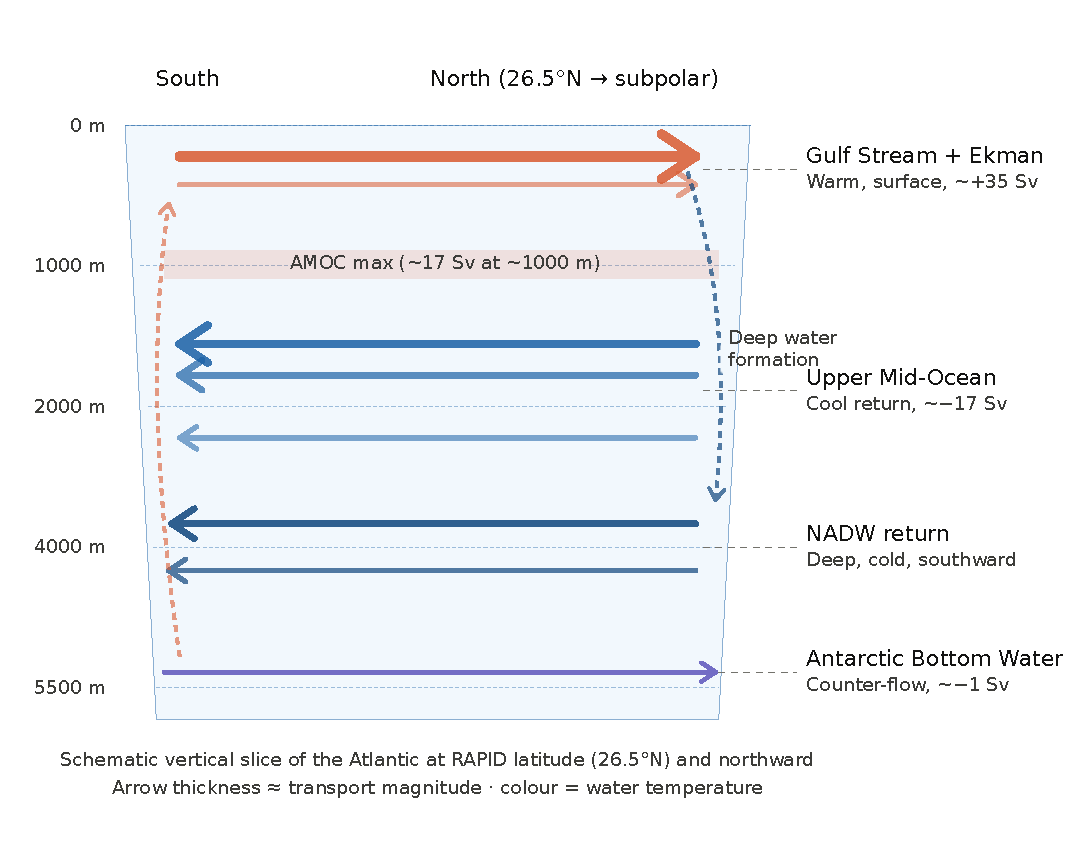
\includegraphics[width=0.9\textwidth]{figures/background/amoc_atlantic_cross_section.pdf}
    \caption[The Atlantic overturning circulation.]{\textbf{The Atlantic
    overturning circulation in cross-section.} Warm surface water flows north
    (magenta), releases heat to the atmosphere in the subpolar seas, grows dense
    and sinks, and returns south as a cold deep current (teal). The vertical
    overturning is driven by density differences of temperature and salinity.
    The circulation has no visible surface expression --- the invisibility the
    thesis sets out to address.}
    \label{fig:amoc-schematic}
\end{figure}

The consequence is climatic, not merely oceanographic. The northward surface flow carries of the order of a petawatt of heat into the North Atlantic --- comparable to the output of a million large power stations --- and much of the relative mildness of northwest Europe depends on it \citep{buckley2016}. Yet the system has no surface that an observer can see: it is a circulation in the ocean's interior, spanning a basin, unfolding over decades. This is precisely the gap the thesis addresses --- a process of great consequence and no everyday visibility.

% -------------------------------------------------------------------------
\section{Bistability and Tipping}
\label{sec:bg-bistability}

What makes the AMOC a \emph{tipping element}, rather than a system that simply weakens in proportion to warming, is a feedback first captured by \citet{stommel1961} in a simple two-box model of the ocean.\footnote{Stommel represented the ocean as two boxes, equatorial and polar, exchanging water at a rate set by their density difference. The salt-advection feedback in his equations yields two stable equilibria for the same external forcing --- the mathematical signature of bistability.} The mechanism is a loop: the overturning carries salt northward, salt keeps northern water dense, and dense water keeps sinking, sustaining the overturning. Add enough freshwater to the North Atlantic --- from melting ice, for instance --- and the loop can run in reverse: fresher water is less dense, sinking weakens, less salt is carried north, and the circulation slows itself further.

Because of this feedback, the AMOC has two stable states --- vigorous overturning, and a much weaker one --- for the same conditions. A gradual push can therefore trigger an abrupt switch, and reversing the push does not simply reverse the switch.% RESTORE WHEN THE FIGURE EXISTS: (Figure~\ref{fig:stommel-hysteresis})
This property, called hysteresis, is why the system's behaviour is non-linear and why it resists intuition: cause and effect are not proportional. Communicating that non-linearity, which no static curve conveys, is the representational challenge at the centre of this thesis.

% -------------------------------------------------------------------------
\section{Measuring the Circulation}
\label{sec:bg-measurement}

To analyse the AMOC, its strength must be expressed as a number. That number is the volume of water the overturning moves, measured in \emph{sverdrups} (\SI{1}{\sverdrup} = \SI{e6}{\cubic\metre\per\second} --- a million cubic metres per second).\footnote{Formally, the overturning streamfunction integrates the northward velocity across the basin and upward from the sea floor; its maximum over depth defines the AMOC transport at a given latitude.} A typical mid-latitude overturning runs at roughly \SIrange{15}{20}{\sverdrup}.

Crucially for what follows, the circulation is not a single number but a \emph{profile}: transport varies with depth, strong near the surface where warm water flows north, reversing at depth where cold water returns south. This vertical profile, resolved over time, is the raw material the \emph{detect} phase decomposes --- the object from which machine learning recovers a compact latent structure in Chapter~\ref{ch:data_pipeline}.

% -------------------------------------------------------------------------
\section{Observational Data}
\label{sec:bg-data}

The AMOC is observed directly by the RAPID-MOCHA-WBTS array (Rapid Climate Change --- Meridional Overturning Circulation and Heatflux Array --- Western Boundary Time Series) at \ang{26.5}~north, a line of moored instruments spanning the Atlantic that has measured the overturning continuously since 2004 \citep{frajkawilliams2021, moat2026}. RAPID is the empirical anchor of this thesis: a genuine, continuous record of a system that had previously been only inferred.

Its one limitation is length. Two decades of data are short against a circulation that varies over decades to centuries, so the observed record cannot alone reveal the system's slow behaviour. To provide longer context, the analysis adds the Copernicus Marine GREP ensemble --- a reanalysis that reconstructs the circulation before the observational period by combining models with assimilated data, at the cost of introducing model dependence and a spread between ensemble members. That spread is not merely a caveat: it becomes, in the \emph{translate} phase, the raw form of uncertainty the representation must make perceptible. Together, observation and reanalysis are the two datasets the next chapter analyses.